\ifdefined\LFSWebBook\else
\documentclass[../textbook.tex]{subfiles}
\begin{document}
\fi
\bookchapter{增量解码}{ch:incremental-decoding-cache}

自回归生成每次只增加少量词元，但新的词元需要读取已经形成的上下文。如果每一步重新执行整个前缀，模型会反复计算相同的位置表示。键值缓存利用因果结构保留这些中间结果，把后续计算集中于新增位置；与此同时，缓存随序列增长，成为并发、显存与状态一致性的核心约束。

缓存复用以因果结构为基础，其存储形式包括连续布局、分页寻址和前缀共享。\bookxref{ch:rev-transformer}定义网络层，\bookxref{ch:long-context}讨论长距离能力。本章侧重执行状态；算子优化和投机生成由\bookxref{ch:inference-algorithms}展开，服务调度由\bookxref{ch:batching-scheduling}展开。

\section{预填充与增量解码}

\subsection{两个阶段的输入输出}
\term{预填充}{Prefill}{}对已知提示的全部位置执行因果前向，形成各层键和值。\term{增量解码}{Incremental Decoding}{}随后只处理新加入的词元，通过历史缓存读取前缀信息。它改变执行方式，自回归概率分解保持不变。

提示包含 $P$ 个词元，编号 $0,\ldots,P-1$。预填充最后位置的输出分布预测第一个生成词元 $y_0$；采样出 $y_0$ 后，才把它送入位置 $P$ 的增量前向，得到预测 $y_1$ 的分布。因而输出 $G$ 个词元通常需要一次预填充与 $G-1$ 次后续单词元前向，而不必为最后一个输出再执行一次模型。\footnote{若服务需要把完整最终回答状态留下用于续聊，可能额外处理最后输出词元。请求返回了多少词元与缓存实际覆盖到哪个位置应分别记录。}

\subsection{张量形状}
设批次大小 $B$，隐藏维数 $d$，层数 $N$，查询头数 $h_q$，键值头数 $h_{kv}$，键维数 $d_k$，值维数 $d_v$。预填充一层有
\begin{equation}
 \mat{H}\in\mathbb R^{B\times P\times d},\quad
 \mat{Q}\in\mathbb R^{B\times h_q\times P\times d_k},\quad
 \mat{K}\in\mathbb R^{B\times h_{kv}\times P\times d_k},\quad
 \mat{V}\in\mathbb R^{B\times h_{kv}\times P\times d_v}.
\end{equation}
若已经缓存 $L$ 个词元，新加入 $\vect{q}$ 个词元，则 $\mat{Q}_{\mathrm{new}}$ 的序列轴为 $\vect{q}$，$\mat{K},\mat{V}$ 的可读取序列轴为 $L+\vect{q}$。单词元解码时 $\vect{q}=1$，每个查询头的注意力分数形状为 $[B,1,L+1]$。实际运行时可采用不同轴顺序或打包布局，逻辑维度不变。

设 $g(i)$ 将查询头 $i$ 映射到其键值头，新增位置 $r\in\{0,\ldots,\vect{q}-1\}$ 的注意力为
\begin{equation}
 \vect{o}_{r,i}=\sum_{j=0}^{L+r}
 \frac{\exp(\frac{\vect{q}_{r,i}^{\top}\vect{k}_{j,g(i)}}{\sqrt{d_k}}+b_{L+r,j})}
 {\sum_{u=0}^{L+r}\exp(\frac{\vect{q}_{r,i}^{\top}\vect{k}_{u,g(i)}}{\sqrt{d_k}}+b_{L+r,u})}
 \vect{v}_{j,g(i)}.
 \label{eq:cache-attn}
\end{equation}
$b$ 表示合法的位置偏置，旋转位置编码则通常已经作用于查询与键。新块内部同样受因果约束 $j\le L+r$ 限制，较早新词元读不到较晚新词元。

\subsection{符号与一致性假设}
\begin{table}[htbp]
\centering
\caption{增量解码与键值缓存主要符号与计量对象}
\label{tab:rev-cache-symbols}
\begin{tabularx}{\linewidth}{lX}
\toprule 符号 & 含义\\\midrule
$P,G,L,q$ & 提示长度、输出词元数、已缓存长度、新增位置数。\\
$N,d,h_q,h_{kv},d_k,d_v$ & 网络层数、隐藏维数及注意力维度。\\
$b_k,b_v$ & 单个键或值元素占用的字节数。\\
$\mathcal C^{(\ell)}$ & 第 $\ell$ 层的键值缓存及其位置元数据。\\
$p_b,\mathcal B$ & 每个物理块容纳的词元数与逻辑块到物理块的映射。\\
$r_c,d_C,d_R$ & 潜变量缓存维数、内容查询/键维数与解耦位置分量维数。\\
\bottomrule
\end{tabularx}
\end{table}

\begin{assumption}[缓存等价的条件]
模型参数、适配器、位置规则和可见性规则固定；网络处于推理模式，旧位置的计算不依赖未来词元。层归一化和前馈变换按位置进行，不以不断扩展的整段序列重新计算全局统计。缓存没有被有损修改，并保留与参考全量前向一致的逻辑位置和输入条件。
\end{assumption}

\section{键值缓存等价性}

\subsection{层级因果性证明}
\term{键值缓存}{Key-Value Cache}{KV Cache}保存各层历史位置的 $K,V$。\begin{proposition}[因果网络的缓存等价性]
在上述缓存等价条件下，追加词元保留历史位置的逐层隐状态，使用历史键值缓存计算新增位置与全量前向具有相同的数学结果。设在长度 $L$ 的前向中，第 $\ell$ 层历史位置 $j<L$ 的隐状态为 $h_j^{(\ell,L)}$。现在追加词元扩展为 $L+q$，则
\begin{equation}
 h_j^{(\ell,L)}=h_j^{(\ell,L+q)},\qquad j<L.
 \label{eq:cache-invariant}
\end{equation}
\end{proposition}
\begin{proof}
第一层之前，旧词元及位置编号相同，嵌入相同。假设某层输入的历史状态相同，则其历史 $Q,K,V$ 相同；因果掩码保证旧位置 $j$ 只读取 $0,\ldots,j$，新增位置不进入求和。于是注意力输出相同，逐位置残差、归一化和前馈结果也相同。对层数归纳，式\eqref{eq:cache-invariant}成立。

计算新增位置时，使用缓存的历史键值与重新计算整个前缀所得到的历史键值相同，新位置本身按同一公式计算，故新增隐状态与输出分布也相同。因果掩码与逐位置计算共同保证缓存复用的数学等价性。

\end{proof}

历史查询通常不必保存，因为以后只需要新位置发出的查询；历史键和值仍将被后续查询读取。跨层不能只保存最后一层缓存：第 $\ell$ 层新查询需要第 $\ell$ 层的历史键值，其表示与其他层不同。

\subsection{等价性条件}
双向编码器的旧位置会读取新增文本，这套追加证明需要另行处理。对编码器—解码器模型，如果编码器输出固定，则交叉注意力的编码器键值可以预先计算；若源文本改变，则这些缓存失效。

推理时仍启用随机丢弃、随长度改变位置缩放、修改适配器或依赖全序列统计的操作，都会破坏旧状态不变的前提。量化缓存、选择性淘汰或近似压缩也会引入额外误差，应作为不同执行模式说明。

数学等价与不同内核的逐位相同是两回事。浮点求和顺序、精度与归约布局都可能带来误差；输出概率接近时，贪心最大值也可能发生离散分叉。验证时先比较同一输入下的分数或概率，再检查误差是否来自浮点归约、掩码或位置处理。

\begin{example}


设模型为单层单头，$d_k=1,d_v=2$。前两个位置的缓存为
\begin{equation}
 k_0=0,\ k_1=\log2,\qquad \vect{v}_0=(1,0),\ \vect{v}_1=(0,2).
\end{equation}
第三个新位置的查询 $q_2=1$，新键 $k_2=\log3$，新值 $\vect{v}_2=(3,3)$。无位置偏置时，分数为 $0,\log2,\log3$，指数为 $1,2,3$，归一化权重为 $\frac{1}{6},\frac{2}{6},\frac{3}{6}$。所以
\begin{equation}
 \vect{o}_2=\frac16(1,0)+\frac26(0,2)+\frac36(3,3)
 =\left(\frac53,\frac{13}{6}\right).
 \label{eq:cache-example}
\end{equation}
全量前向会为第三行生成完全相同的分数；缓存前向复用前两行键值即可，前两行的注意力输出始终保留在缓存中。若错误漏掉新键值，得到 $(\frac{1}{3},\frac{4}{3})$，差异由可见集合改变产生。

\begin{figure}[htbp]
\centering
\begin{tikzpicture}[>=stealth,node distance=8mm,every node/.style={font=\small},box/.style={draw,rounded corners,align=center,text width=29mm,minimum height=10mm}]
\node[box] (old){历史 $K_{0:L},V_{0:L}$\\各层已计算};
\node[box,below=of old] (new){新词元隐状态\\生成 $q_L,k_L,v_L$};
\node[box,right=of old] (join){读取历史并追加\\$K_{0:L+1},V_{0:L+1}$};
\node[box,right=of join] (attn){新查询注意力\\残差与前馈};
\node[box,below=of attn] (out){下一层新状态\\最终分布};
\draw[->] (old)--(join);\draw[->] (new)--(join);\draw[->] (join)--(attn);
\draw[->] (new.east)--++(.3,0)-|(attn.south);\draw[->] (attn)--(out);
\end{tikzpicture}
\caption{单层增量计算的数据流。新查询读取全部合法键值，历史查询和历史前馈输出不再重算。}
\label{fig:cache-incremental}
\end{figure}
\end{example}

\section{复杂度与带宽}

\subsection{重复前缀与缓存执行}
忽略层数等固定系数，以密集网络常见维度关系计，长度 $L$ 的全量前向约为 $O(Ld^2+L^2d)$。如果生成每个词元都重算整个前缀，$G$ 次预测消耗约
\begin{equation}
 \sum_{g=0}^{G-1}O\big((P+g)d^2+(P+g)^2d\big).
 \label{eq:cache-naive}
\end{equation}
使用缓存后，预填充一次，后续 $G-1$ 次单词元前向各为 $O(d^2+(P+g)d)$，总量为
\begin{equation}
 O(Pd^2+P^2d)+O\big(Gd^2+(GP+G^2)d\big).
 \label{eq:cache-complexity}
\end{equation}
因此无初始长提示时，朴素重复前缀的注意力累计量可达三次方，而缓存把它降到二次方；单步解码的密集注意力仍随上下文线性增长。

例如提示4个词元、输出3个词元。全量方案分别处理长度4、5、6，累计线性变换位置15个；缓存方案处理4个提示与2个新增位置，共6个。按因果合法分数对计，前者为 $10+15+21=46$，后者为 $10+5+6=21$。端到端耗时还取决于运算类型、内核和访存。

\subsection{缓存容量与计算量}
单步解码需要读取历史键值。若主要限制是显存带宽，减少缓存元素有助于降低读取成本；但查询头数不变时，注意力分数与输出仍按查询头计算。预填充可以对许多查询并行执行，单词元解码更容易受参数与缓存读取影响，两个阶段各有自己的吞吐常数。

缓存复用历史键值，新词元仍需执行网络层计算并读取可见上下文。实际耗时还取决于批次、内核复用、页布局、并行通信和工作区；\bookxref{ch:inference-algorithms}讨论算子，\bookxref{ch:batching-scheduling}讨论调度。容量预算与负载下的延迟测量共同用于服务规划。

\section{MHA、GQA 与 MQA 的缓存}

\subsection{头共享结构}
\term{多头注意力}{Multi-Head Attention}{MHA}为每个查询头提供独立键值头，$h_{kv}=h_q$。\term{多查询注意力}{Multi-Query Attention}{MQA}让所有查询头共享一个键值头，$h_{kv}=1$\cite{shazeer2019mqa}。\term{分组查询注意力}{Grouped-Query Attention}{GQA}在两者之间按组共享键值\cite{ainslie2023gqa}。

若 $h_q$ 能被 $h_{kv}$ 整除，每组有 $\frac{h_q}{h_{kv}}$ 个查询头。共享键值时，各查询向量仍可产生不同的注意力权重。MHA、GQA 与 MQA 具有不同的参数化结构，结构转换通常需要相应训练与质量评估。

\begin{figure}[htbp]
\centering
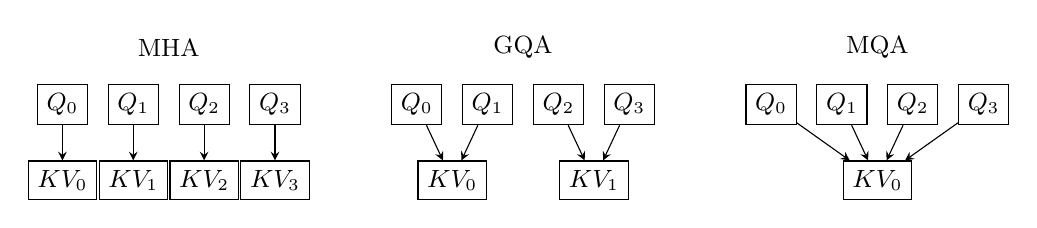
\begin{tikzpicture}[x=.9cm,y=.8cm,>=stealth,every node/.style={font=\small}]
\foreach \base/\title in {0/MHA,5/GQA,10/MQA}{
 \node at (\base+1.5,1.5){\title};
 \foreach \i in {0,1,2,3}{\node[draw] (q\base\i) at (\base+\i,.6){$\mat{Q}_{\i}$};}}
\foreach \i in {0,1,2,3}{\node[draw] (k0\i) at (\i,-.6){$\mat{K}\mat{V}_{\i}$};\draw[->] (q0\i)--(k0\i);}
\node[draw] (g0) at (5.5,-.6){$\mat{K}\mat{V}_0$};\node[draw] (g1) at (7.5,-.6){$\mat{K}\mat{V}_1$};
\draw[->] (q50)--(g0);\draw[->] (q51)--(g0);\draw[->] (q52)--(g1);\draw[->] (q53)--(g1);
\node[draw] (m0) at (11.5,-.6){$\mat{K}\mat{V}_0$};\foreach \i in {0,1,2,3}{\draw[->] (q10\i)--(m0);}
\end{tikzpicture}
\caption{四个查询头下的键值共享关系。查询头数相同，缓存键值头数依次为4、2、1。}
\label{fig:cache-heads}
\end{figure}

\subsection{统一容量公式}
若请求 $b$ 缓存长度为 $L_b$，各层同形状，则裸缓存容量为
\begin{equation}
 M_{KV}=N\sum_bL_bh_{kv}(d_kb_k+d_vb_v).
 \label{eq:cache-memory}
\end{equation}
当 $d_k=d_v=d_h,b_k=b_v=b_e$、所有请求长度 $L$ 相同时，退化为 $2NBLh_{kv}d_hb_e$。它不包含页表、分配碎片、量化比例、临时空间和模型权重。分层采用滑窗或不同头数时，应分别求和。

取 $N=32,h_q=32,d_h=128,b_e=2,L=8192,B=1$。每词元 MHA 缓存为 $2\times32\times32\times128\times2=524288$ 字节，即512 KiB。GQA 取8个键值头，每词元128 KiB；MQA 每词元16 KiB。如表\ref{tab:rev-cache-variants-memory}所示，不同架构的裸 KV 缓存显存占用存在数量级差异。

\begin{table}[htbp]
\centering
\caption{不同注意力架构在典型配置下的裸 KV 缓存显存占用对比}
\label{tab:rev-cache-variants-memory}
\begin{tabular}{lrrr}
\toprule 结构 & 键值头数 & 单请求裸缓存 & 四请求裸缓存\\\midrule
MHA & 32 & 4 GiB & 16 GiB\\
GQA & 8 & 1 GiB & 4 GiB\\
MQA & 1 & 128 MiB & 512 MiB\\
\bottomrule
\end{tabular}
\end{table}
这里 GiB 为 $2^{30}$ 字节。模型总显存还包括权重与工作区，吞吐还受计算、带宽和调度影响。

张量并行下，若键值头均匀分片，每卡缓存可相应减少；若键值头少于并行设备数而运行时复制，直接除以并行度会低估每卡占用。例如 MQA 的一个头可能在多个设备上分别驻留。容量规划需使用实际每卡存储头数，并与模型及内核布局一致。

\section{低秩键值与潜变量缓存}
\optional
\subsection{联合表示与矩阵吸收}
键值头共享减少独立头数，另一种思路是让键和值由低维共同变量生成。对单位置列向量 $\vect{h}_t\in\mathbb R^d$，设
\begin{equation}
 \vect{c}_t=\mat{W}_D\vect{h}_t\in\mathbb R^{r_c},\quad
 \vect{k}_{t,i}=\mat{U}_{K,i}\vect{c}_t,\quad \vect{v}_{t,i}=\mat{U}_{V,i}\vect{c}_t,
\end{equation}
其中 $\mat{U}_{K,i}\in\mathbb R^{d_k\times r_c}$，$\mat{U}_{V,i}\in\mathbb R^{d_v\times r_c}$。不含位置旋转时
\begin{equation}
 \vect{q}_{t,i}^{\top}\vect{k}_{j,i}=(\mat{U}_{K,i}^{\top}\vect{q}_{t,i})^{\top}\vect{c}_j.
 \label{eq:cache-absorb-key}
\end{equation}
可以先把当前查询投到潜空间，再与缓存 $\vect{c}_j$ 点积，不必为每个历史位置展开完整键。输出也有
\begin{equation}
 \sum_j a_{t,j,i}\vect{v}_{j,i}=\mat{U}_{V,i}\sum_j a_{t,j,i}\vect{c}_j.
\end{equation}
若第 $i$ 头输出投影块为 $O_i$，可进一步合并 $O_i\mat{U}_{V,i}$。这种\term{矩阵吸收}{Matrix Absorption}{}利用线性结合与矩阵乘法结合律，改变计算顺序而保留所定义低秩结构的数学结果。

低秩结构约束键值投影的表示空间。模型若按该结构训练，可以精确执行自身的潜变量形式；若对已有高秩权重作事后低秩近似，则还需分析近似误差。缓存变小也可能增加某些潜空间计算，必须结合维度与执行阶段权衡。

\subsection{位置旋转的非交换约束}
若对完整键加入旋转 $\mat{R}_j$，查询也按位置 $t$ 旋转，则点积为
\begin{equation}
 \vect{q}_{t,i}^{\top}\mat{R}_t^{\top}\mat{R}_j\mat{U}_{K,i}\vect{c}_j.
\end{equation}
中间旋转依赖历史位置 $j$，吸收到当前查询投影需要一个与 $j$ 无关的固定矩阵，这样的矩阵一般并不存在。矩阵通常不交换次序；忽略这一点会把缓存压缩推导变成错误等式。

\term{多头潜在注意力}{Multi-Head Latent Attention}{MLA}在 DeepSeek-V2 中采用联合键值压缩与解耦位置分量\cite{deepseek2024v2}。概念上可把分数写为内容项和位置项之和：
\begin{equation}
 s_{t,j,i}=\frac{(\vect{q}^C_{t,i})^\top \mat{U}_{K,i}\vect{c}_j+
 (\vect{q}^R_{t,i})^\top \vect{k}^R_j}{\sqrt{d_C+d_R}}.
 \label{eq:cache-mla}
\end{equation}
内容项采用矩阵吸收，旋转位置项单独保留。分母与该结构的查询、键总维度和训练尺度一致，换成潜变量维数会破坏这一对应。这里只给出缓存相关关系，具体查询压缩与模型规格应遵循对应架构。

若每层每位置保存一个 $r_c$ 维潜变量和一个共享 $d_R$ 维位置键，统一元素字节数 $b_e$ 时，裸容量为
\begin{equation}
 M_{\mathrm{latent}}=N\sum_bL_b(r_c+d_R)b_e.
\end{equation}
例如取 $r_c=512,d_R=64,N=32,b_e=2,L=8192$，得到288 MiB。缓存容量由潜变量维度、位置键维度、层数、序列长度和元素精度共同决定。

\section{逻辑位置与物理分页}

\subsection{页表不改变注意力位置}
\term{分页键值缓存}{Paged KV Cache}{}把序列的连续逻辑位置映射到可不连续的物理块。PagedAttention 将此思路用于模型服务中的缓存管理\cite{kwon2023pagedattention}。若每块容纳 $p_b$ 个词元，逻辑位置 $t$ 对应
\begin{equation}
 j=\lfloor \frac{t}{p_b}\rfloor,\qquad o=t\bmod p_b,
 \qquad \mathrm{physical}(t)=(\mathcal B[j],o).
 \label{eq:cache-page}
\end{equation}
$j$ 为逻辑块编号，$o$ 为块内偏移，$\mathcal B$ 是请求页表。位置编码仍使用逻辑位置 $t$，物理块编号只描述存储位置。搬迁一个块只需更新映射与数据位置，不应重新解释序列顺序。

设块大小4、逻辑长度10，页表为 $(7,2,9)$。位置6映射到物理块2的偏移2，位置9映射到物理块9的偏移1。三个物理块共有12个槽位，最后两位无效，注意力必须根据逻辑长度排除它们。

\begin{figure}[htbp]
\centering
\begin{tikzpicture}[>=stealth,every node/.style={font=\small},b/.style={draw,minimum width=28mm,minimum height=8mm,align=center}]
\node[b] (l0) at (0,1){逻辑0--3};\node[b] (l1) at (0,0){逻辑4--7};\node[b] (l2) at (0,-1){逻辑8--9};
\node[b] (p2) at (4,1){物理块2};\node[b] (p7) at (4,0){物理块7};\node[b] (p9) at (4,-1){物理块9};
\draw[->] (l0)--(p7);\draw[->] (l1)--(p2);\draw[->] (l2)--(p9);
\node[align=left] at (8,0){位置6：块2，偏移2\\位置9：块9，偏移1\\位置编码仍为6、9};
\end{tikzpicture}
\caption{逻辑块映射到不连续物理块。页表解决存储布局，逻辑位置和有效长度决定模型可见的内容。}
\label{fig:cache-pages}
\end{figure}

\subsection{碎片与容量预留}
没有共享时，请求长度 $L_b$ 需要 $\lceil \frac{L_b}{p_b}\rceil$ 个块，分配槽位与有效长度之差小于 $p_b$。对 $B$ 条请求，尾部内部碎片少于 $Bp_b$ 个词元槽位。块太大增加尾部浪费，块太小增加页表和寻址开销，选择应结合内核与长度分布。

缓存按需增长减少一次预留最大输出长度的浪费，后续增长风险仍然存在。接纳请求时应考虑未来输出预算及可用块；正在执行的内核读取旧映射期间，块不能被提前回收。页表修改、数据拷贝与设备执行之间需要明确顺序和完成边界。

\subsection{批内变长}
对长度分别为 $L_1,\ldots,L_B$ 的请求，每个新查询仅能读取自身有效前缀。连续批次中的行号只是当前执行槽位，与稳定请求身份是两回事。请求完成后压缩批次、交换行或加入新请求时，缓存映射必须跟随请求，原行对应的物理块不再自动适用。

填充到批内最大长度的实现与分页变长实现可以表达同一逻辑计算；前者需要屏蔽无效位置，后者需要正确页表与长度。它们的缓存分配量和算子效率不同，语义保持一致。

\section{前缀共享与缓存生命周期}

\subsection{计算前缀共享}
\term{前缀缓存}{Prefix Cache}{}复用多个请求相同前缀产生的键值。因为旧状态只依赖前面的内容，相同模型、相同逻辑位置与相同条件下的精确词元前缀可以共享。相同的一段后缀若前文不同，深层键值通常不同，只按局部文本匹配会误判复用条件。

共享通常从完整块边界开始。前缀块的身份应绑定前一块身份与本块词元内容，使同一局部块出现在不同前缀后时不被误判为相同计算状态。内容摘要是索引手段，仍需要足够可靠的身份方案与兼容性元数据。

完整命中提示缓存时，首个新词元的采样还需要最后位置的隐状态或输出分数。实现可以保留相应输出状态，或重新处理最后一个提示位置并精确控制缓存截断与追加。重新处理时应覆盖对应位置，保持前缀长度与输出状态一致。

\subsection{引用计数与写时复制}
共享块在被多个请求引用时应保持不可变。\term{引用计数}{Reference Counting}{}记录有多少活动使用者持有该物理块；释放一个请求只减少其引用，计数归零后才具备回收条件。若块仍被设备内核读取，还需等待相关执行完成。

当多个分支共享未满块又要追加不同词元时，需要\term{写时复制}{Copy-on-Write}{CoW}：为修改分支分配新块，复制有效前缀，再追加。否则一个请求会覆盖另一个请求的缓存。已满共享块无需复制，后续分支直接分配各自的新块即可。

例如每块4个词元，三条请求共享8个前缀词元，各自拥有3个后续词元。独立存储需要 $3\times\lceil\frac{11}{4}\rceil=9$ 块；共享后需要2个公共块加3个私有尾块，共5块。有效独特缓存词元为 $8+3\times3=17$，分配20槽位；节省的是重复前缀，私有后缀仍各自计算。

\subsection{缓存驻留与淘汰}
对活动请求正在使用的缓存，“最近没访问”不构成删除理由。\term{缓存淘汰}{Cache Eviction}{}通常针对没有活动引用但为未来复用保留的块；若要抢占活动请求，应保存可恢复映射并换出，或释放后按同一输入重新计算。前者消耗传输，后者消耗计算，两者的语义与普通缓存命中不同。

缓存可经历空闲、分配写入、可共享驻留、活动引用、无引用可淘汰、回收等状态。取消与超时也必须走释放路径，并以请求资源所有权防止重复递减。前缀复用率高但长期占满显存时，驻留策略会挤压活动解码；如何在任务之间分配资源由调度章节展开。

\begin{figure}[htbp]
\centering
\begin{tikzpicture}[>=stealth,every node/.style={font=\small},b/.style={draw,rounded corners,align=center,text width=2.5cm,minimum height=.8cm}]
\node[b] (free) at (0,0) {空闲物理块};
\node[b] (write) at (4,0) {私有写入\\尚未发布};
\node[b] (active) at (8,0) {已提交、活动引用\\共享内容不可变};
\node[b] (resident) at (8,-2.3) {无活动引用驻留\\等待或可淘汰};
\draw[->] (free)--node[above]{分配}(write);
\draw[->] (write)--node[above]{完成并提交}(active);
\draw[->] (active)--node[right]{最后引用释放}(resident);
\draw[->] (resident.east) to[bend right=35] node[right]{命中、取引用} (active.east);
\draw[->] (resident.west)--node[below,align=center]{淘汰：引用为零且设备使用结束}(0,-2.3)--(free);
\draw[->,dashed] (write.south)--(4,-1.2)-|node[pos=.25,below]{写入失败，完成回滚}(free.south);
\draw[->,dashed] (active.north) to[bend right=35] node[above]{CoW：分配新块并复制} (write.north);
\end{tikzpicture}
\caption{缓存块生命周期。CoW边表示创建新的私有副本，原共享块仍保持原状态；取消与正常结束都按所有权释放一次引用。未完成的设备访问禁止复用物理存储。}
\label{fig:cache-lifecycle}
\end{figure}

\begin{algorithm}[前缀缓存的引用与追加]
输入为计算身份、词元前缀、请求身份及所需新增容量；输出为请求页表和可继续执行的私有尾部。
\begin{enumerate}
\item 在允许共享的命名空间内查找最长兼容完整前缀，逐块验证计算身份与有效范围，取得引用后固定映射。
\item 为未命中部分分配块，执行预填充并提交有效长度；只有计算完成的内容可发布为可共享状态。
\item 每次追加前判断尾块是否有空位及是否被共享；共享且需要修改时先复制有效内容到私有块。
\item 写入各层新键值，在成功完成后推进逻辑长度；失败时回滚未提交分配，不发布部分完成状态。
\item 请求终止后按所有权恰好释放一次引用；待无引用且设备使用结束后，块可保留驻留或由淘汰策略回收。
\end{enumerate}
不变量是任何活动页表只能指向兼容且已完成的有效数据，共享块不被原地覆盖，逻辑长度只描述已提交状态。
\end{algorithm}

\section{滑窗、淘汰与位置编码约束}

\subsection{历史状态淘汰条件}
模型若原本采用包含当前位置的窗口 $w$，未来查询只读取最近 $w$ 个键值，则窗口之外的历史键值不再作为该层的直接输入，可在保持必要元数据的条件下回收。删除全注意力模型的旧键值，则改变式\eqref{eq:cache-attn}的求和集合，属于近似策略。表\ref{tab:rev-kv-compression-taxonomy}梳理了工业界与学术界主流的 KV 缓存压缩与显存优化技术全景。

\begin{table}[htbp]
\centering
\small
\setlength{\tabcolsep}{3.5pt}
\caption{大语言模型 KV 缓存压缩与显存优化技术全景对比}
\label{tab:rev-kv-compression-taxonomy}
\begin{tabularx}{\linewidth}{lp{22mm}ccX}
\toprule
技术路线 & 代表方案 & 理论压缩比 & 精度影响 & 核心机制与工程权衡 \\
\midrule
头维度共享 & MQA / GQA & $2\times\sim 8\times$ & 极低（需预训） & 减少独立键值头数，极大降低访存带宽压力 \\
低秩潜在投影 & MLA (DeepSeek) & 约 $4\times\sim 7\times$ & 极低（原生） & 潜变量投影结合解耦 RoPE，兼顾容量与显存 \\
存储分页管理 & PagedAttention & 碎片降至 $<4\%$ & 无损 & 离散虚拟分页，彻底根除预留长度的显存碎片 \\
低比特量化 & FP8 / INT4 KV & $2\times\sim 4\times$ & 需离群保护 & 词元/通道量化，大幅提升并发批处理吞吐 \\
局部窗口截断 & StreamingLLM & 上限 $\mathcal{O}(W)$ & 损长程依赖 & 保留少量初始注意力沉点与局部滑动窗口 \\
稀疏注意力 & H2O / SnapKV & 约 $2\times\sim 5\times$ & 取决于检索需求 & 依据注意力得分动态淘汰冗余历史键值 \\
\bottomrule
\end{tabularx}
\end{table}

滑窗模型的高层新状态可能包含通过中间位置传递的更早信息。缓存中仅保留最近键值，与从原始文本只取最近 $w$ 个词元重新运行整网是两种不同的计算：后者可能失去这些键值形成时曾使用的上下文。精确性应相对于相同逐步滑窗计算定义。

混合全局层与滑窗层时，缓存保留范围按层不同。用于前缀匹配的累计逻辑长度与当前驻留位置数是两个量，应同时保存历史进度和各层可见范围。

\subsection{环形存储的逻辑位置}
\term{环形缓存}{Ring Buffer}{}用位置 $t\bmod w$ 复用物理槽位。槽位编号是存储坐标，位置编码仍应使用模型定义的逻辑位置 $t$。把槽位0当成绝对位置0，会改变旋转相位或绝对嵌入。

如果缓存保存已经旋转的键，移动物理块不需要重新旋转；若改变逻辑位置，情况不同。纯相对旋转在特定条件下可以通过一致变换分析重定位，但普通网络还包含深层上下文状态，只改键相位还不足以让任意裁剪与拼接等价。

长度扩展方案若根据当前长度动态修改旋转频率，旧键以及形成旧键的深层状态可能不再对应新规则。最稳妥的缓存复用前提是一次请求内固定位置配置；需要动态改变时应明确重建范围，只更新配置数字不够。

\section{缓存身份与隔离}

\subsection{缓存失效依赖}
缓存是给定计算条件的中间结果。其身份至少应覆盖权重及结构修订、适配器组合、精度与缓存格式、位置配置、注意力规则、精确前缀和外部条件。对多模态或交叉注意力模型，还需绑定媒体特征、处理器和编码器状态；图像条件由对应的媒体特征与编码状态确定。

分词器与模板决定如何得到词元前缀，适合在制品身份中统一绑定。温度与采样阈值若仅作用于输出分布而不改变前向，本身不改变已有前缀 KV；但它们影响后续采样结果及恢复随机轨迹，因此仍属于请求生成状态。区分这两类依赖可以避免缓存键过宽或过窄。

模型身份使用确定的权重与结构修订。更新模型而继续使用旧缓存会得到混合版本计算；同一个请求在解码中切换修订也不具有普通续算语义。无损搬迁到相同制品通常只改变位置，跨不同缓存布局则需要明确定义格式转换。

\subsection{多租户共享边界}
缓存包含由用户内容计算出的状态，应受请求或授权共享域控制。跨租户复用需要对应共享域的授权。命名空间、前缀来源和授权域应进入查找边界；公共固定前缀可以在明确规则下共享，私有内容的访问范围不因摘要命中而扩大。

引用计数管理内存生命周期，授权域管理访问范围。缓存命中造成的时间差、日志或错误信息也可能泄露前缀存在性，应避免向无权请求暴露可查询的私有前缀信息。物理块重新分配后，旧内容必须在访问与有效长度上不可见，并在复用前建立新的有效范围。

\begin{note}[缓存正确性的三个层次]
数学层保证保存的状态等价于相同前缀计算；存储层保证页表、有效长度与生命周期一致；隔离层保证只有授权请求能够复用状态。这三层共同保证缓存复用的正确性。
\end{note}

\section{增量执行过程}

\begin{algorithm}[带缓存的自回归生成]
输入为非空提示、冻结模型、生成上限 $G>0$、停止规则与空或兼容前缀缓存；输出为最多 $G$ 个词元及最终缓存进度。
\begin{enumerate}
\item 确定提示词元、逻辑位置和缓存身份，复用合法前缀并处理未缓存部分，取得提示末位置的输出分布。
\item 根据生成策略选择下一个词元并记录输出；若达到结束条件或输出上限，终止生成。
\item 为该新词元分配可写位置，按层计算新查询、键和值，查询所有合法历史位置并完成残差与前馈；提交缓存及逻辑长度。
\item 从最终层取得下一词元分布，返回步骤2；批内其他请求使用各自页表、长度及终止状态。
\item 正常结束、取消或失败时释放请求持有的资源；若保留续聊状态，明确缓存是否已经覆盖最后输出词元。
\end{enumerate}
每次循环至多增加一个已输出词元，缓存只覆盖已经执行前向的位置；采样后经过前向计算的词元才写入各层 KV。
\end{algorithm}

时间指标也应遵循阶段语义。首词元延迟从约定入口到首个可见输出，通常包含排队与预填充；后续词元间隔描述增量阶段及其排队、传输影响。若 TTFT 已含排队，端到端时间写为 $\mathrm{TTFT}+(G-1)\mathrm{TPOT}$，排队在式中只计一次。缓存命中减少预填充计算，其对首词元延迟的影响还取决于排队与传输。

\section{缓存计量与服务边界}

缓存增长、头共享和容量计数描述状态存储的成本；内核分块、编译与并行效率在后续章节展开。请求身份、模型修订、取消和资源释放决定缓存生命周期与隔离边界。




\chapterreferences
\lfsendchapterdocument
